\section{实时流体渲染算法}
    本文中流体模拟的结果是粒子集,如果直接进行渲染,势必会得到凹凸不平的流体表面,真实感会大大下降。如果是离线渲染,可以使用移动立方体方法\cite{LC87MC}重建流体表面的高精度三角网格,再进行着色。显然这种方法不适用于实时渲染,所以本章设计了一套基于屏幕空间的动态流体渲染解决方案,在性能和资源受限的浏览器环境仍能高效渲染出可以接受的流体效果。

    \begin{figure}[htbp]
    	\centering
    	\includegraphics[width=.9\textwidth]{figures/rendering/raw_filterd.png}
    	\caption{流体粒子仿真结果与流体渲染效果}
    \end{figure}

\subsection{方法概述}
    屏幕空间方法法是实时渲染中的常用的一类方法,比如延迟渲染(Deffered Shading)、屏幕空间环境光遮蔽(Screen-Space Ambient Occlusion)、屏幕空间反射(Screen-Space Reflection)等。它指的是将场景光栅化之后,得到屏幕空间每个像素的几何与材质信息(法向、深度、反照率等),并将它们保存在多个帧缓冲之中(G-Buffer),再利用这些数据进行着色或其他光照计算。屏幕空间方法的复杂度仅与帧缓冲的分辨率有关,与场景复杂度无关,这使得它非常高效,并且适用于各种渲染管线。
    
    本章的流体渲染方案也以屏幕空间方法为基础\cite{G10SSF},首先将粒子实例化渲染,得到两张帧缓冲,分别保存流体表面深度与流体厚度,再对深度图进行平滑,最后进行光线着色。

\subsection{粒子实例化渲染}
    对于单个粒子,本章将其作为广告牌(Billboard)\cite{AHH19RTR}对象进行渲染。所谓广告牌就是固定朝向相机的贴图矩形。与球形网格相比,广告牌仅需两个三角形就可以表示一个粒子,大大减少了性能开销。同时,实验中利用硬件实例化技术渲染所有流体粒子,大大减少Drawcall数量,降低CPU与GPU通信开销。
    
    在着色器的具体实现上,首先根据uv值即可确定像素在矩形广告牌上的位置,如果在球体表面之外则直接丢弃,接下来计算流体表面的屏幕空间坐标,进而得到深度与厚度值。在计算深度图时,渲染管线开启深度测试。而在计算厚度图时,渲染管线关闭深度测试,并开启透明度混合,将着色器输出的厚度值利用硬件进行高效累加,得到每个像素对应流体的总厚度。

    \begin{figure}
    	\centering
    	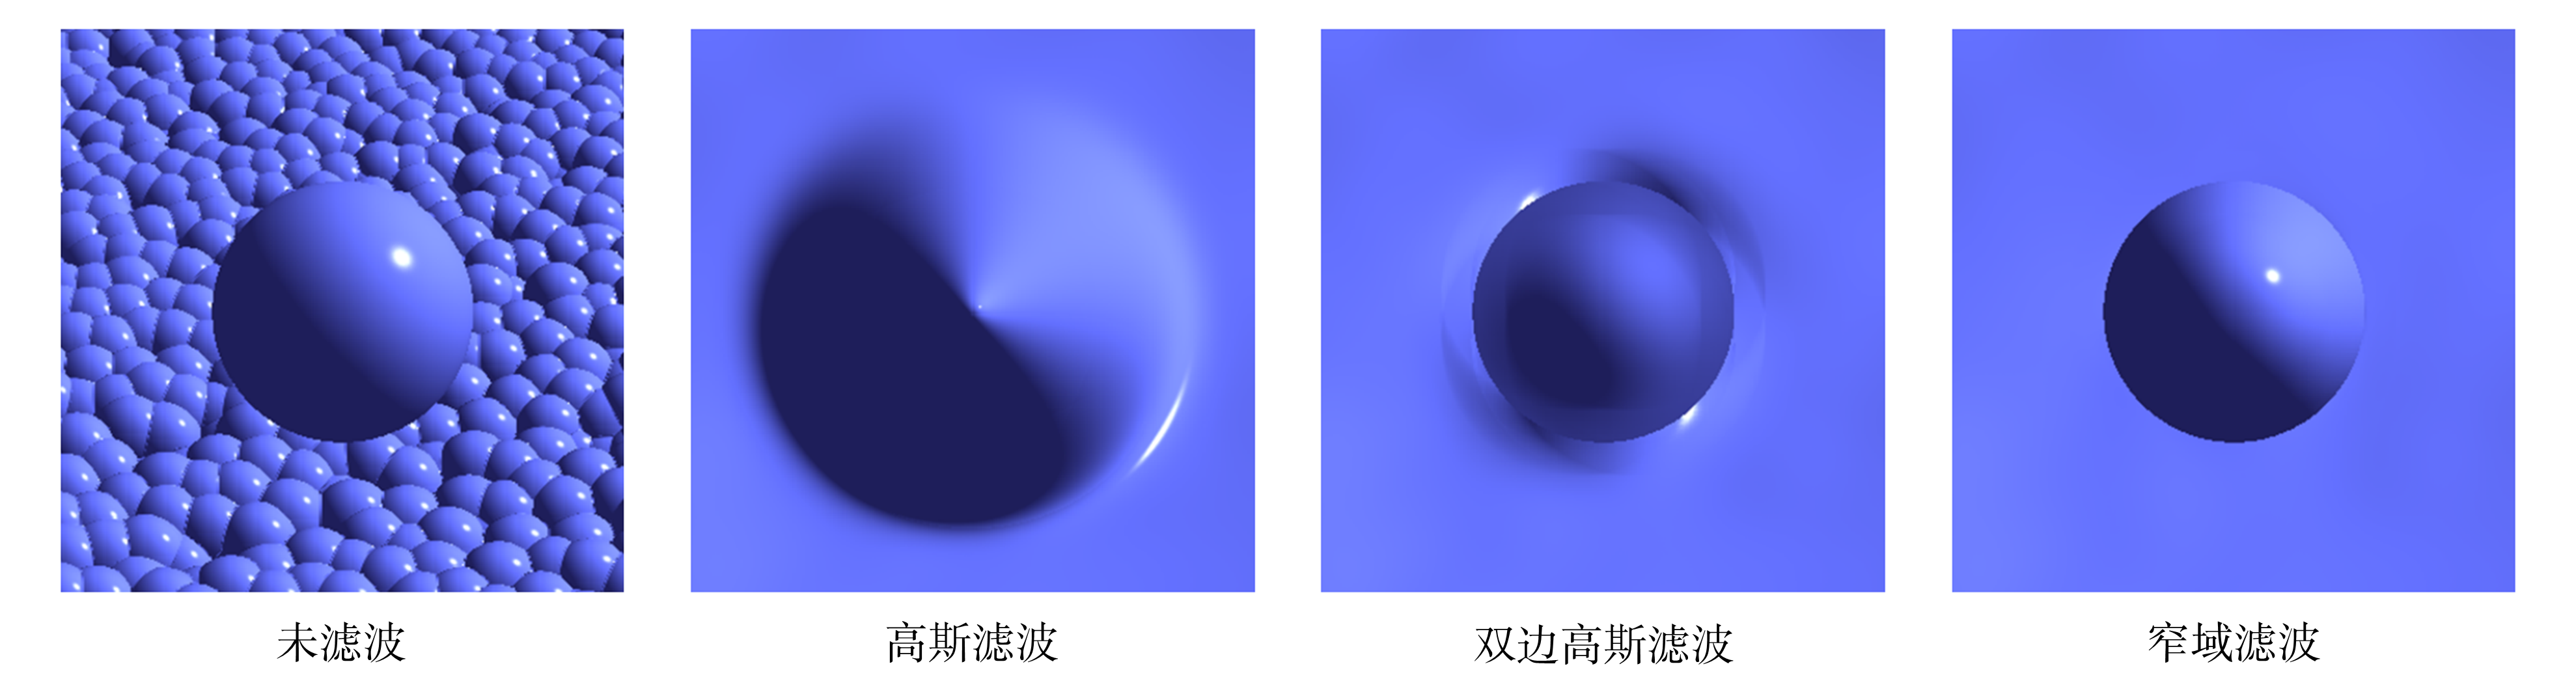
\includegraphics[width=.99\textwidth]{figures/rendering/filters.png}
    	\caption{不同滤波器滤波效果对比\cite{TY18NRSSF}}
    \end{figure}
    
    \begin{figure}
    	\centering
    	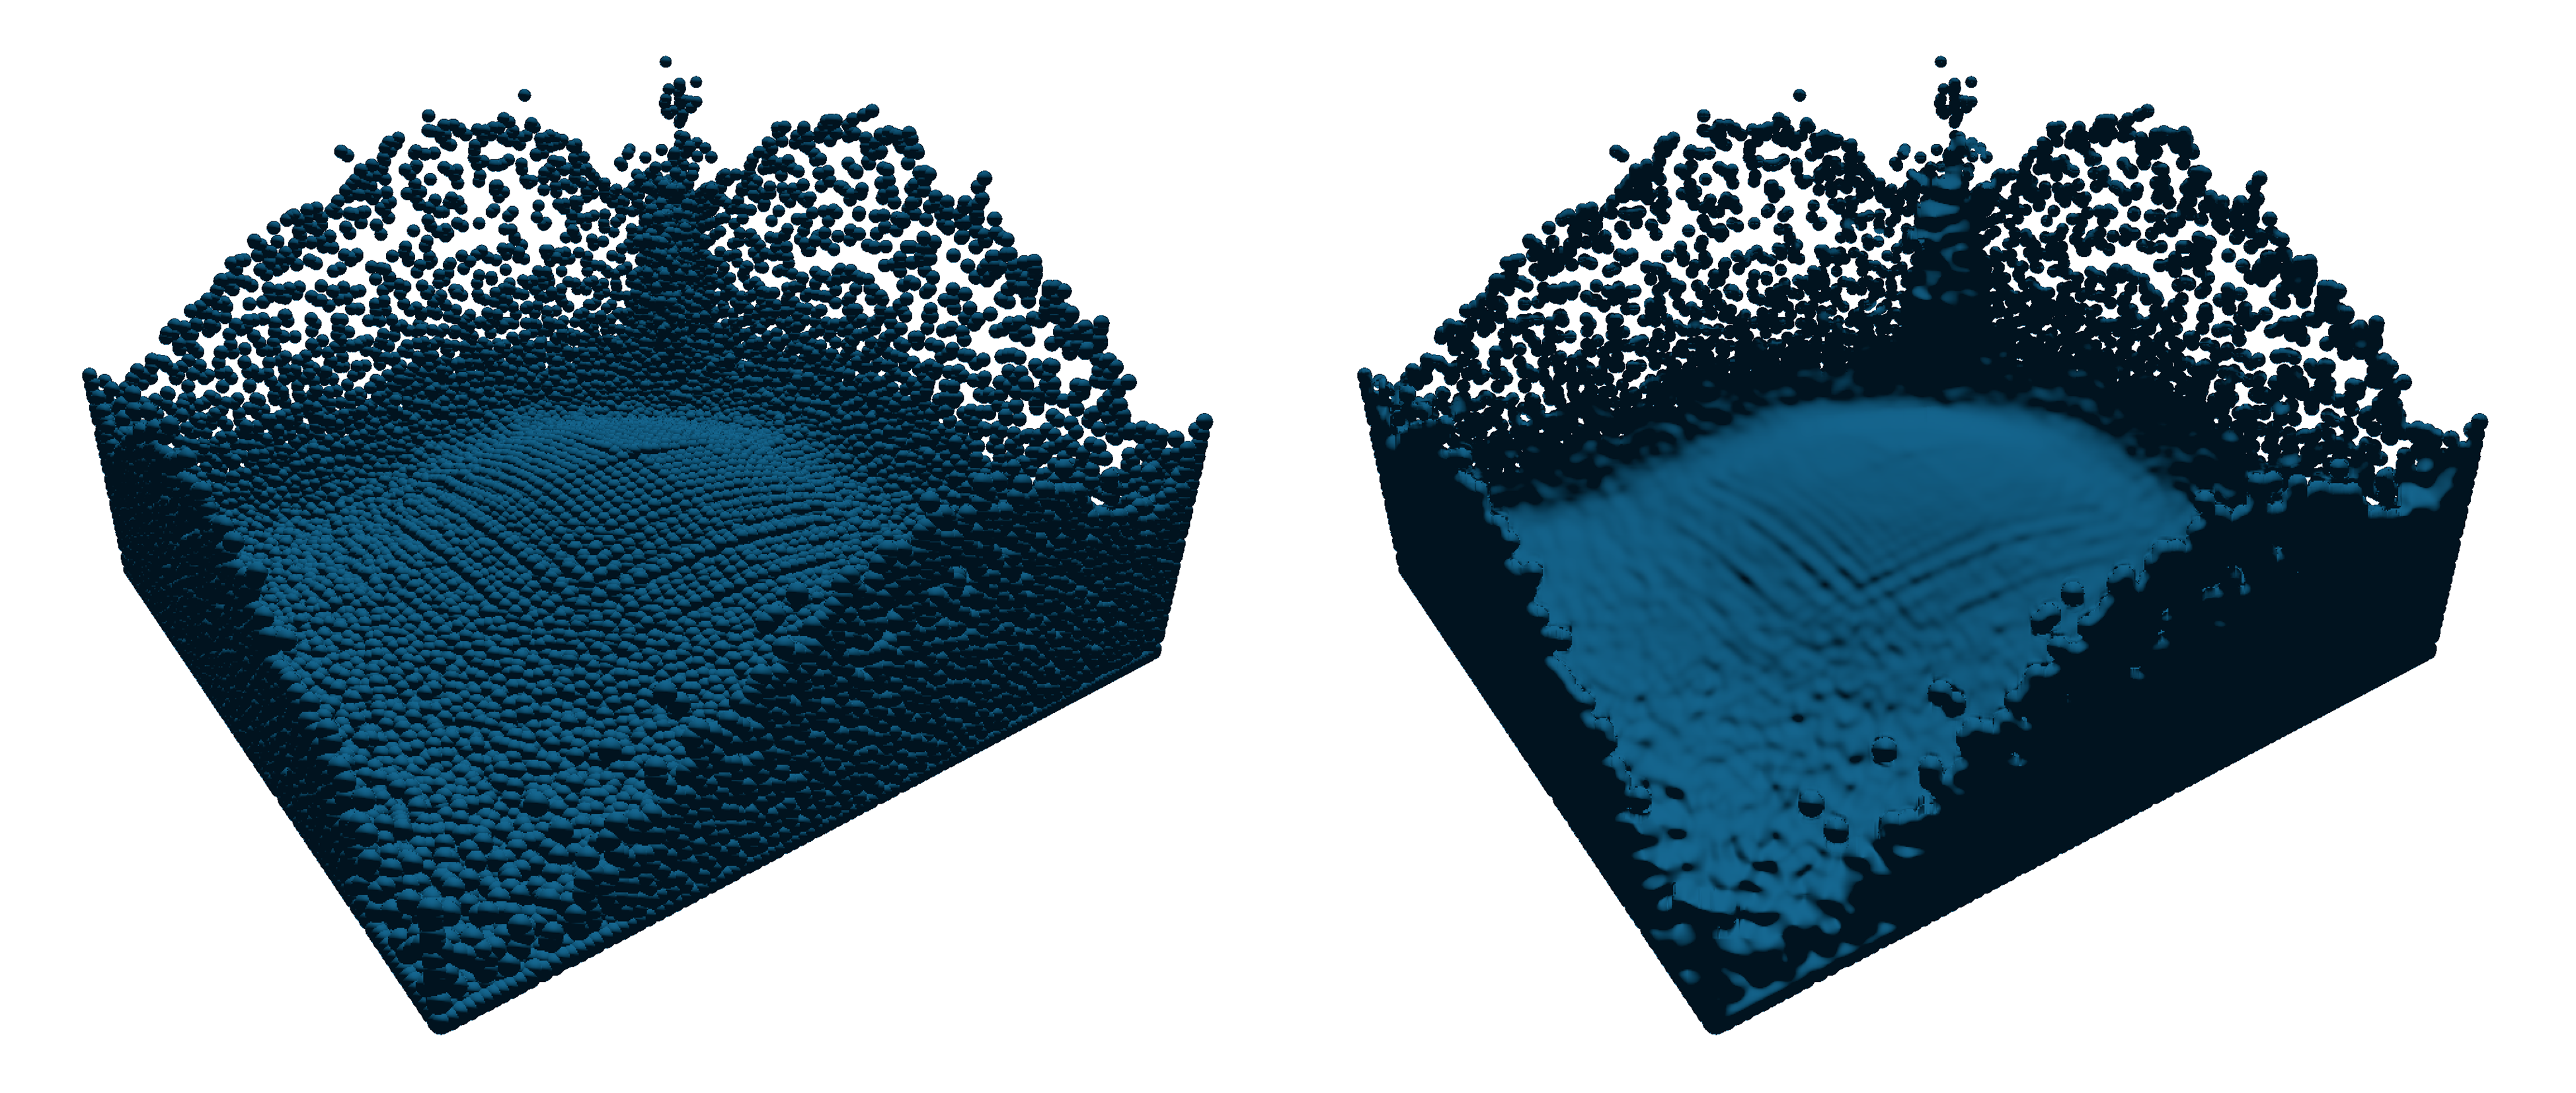
\includegraphics[width=.75\textwidth]{figures/rendering/before_after_filter.png}
    	\caption{深度滤波效果}
    \end{figure}

\subsection{深度图平滑}
    深度图平滑是提高流体渲染真实感的关键步骤。最直接的处理方式是高斯模糊,但这样会融合深度差异过大的表面,使得流体着色结果丢失轮廓边界。Green\cite{G10SSF}提出使用双边高斯滤波,能够有效保留表面轮廓,但是依然会导致边界附近深度值计算出现偏差。Truong等人\cite{TY18NRSSF}进一步提出了窄域滤波(Narrow-Range Filter),解决了双边滤波产生的问题。
    
    所谓窄域,指的是将待滤波的采样点深度值约束在一定范围内,减少深度差异过大的采样点影响滤波结果。窄域滤波的定义为
    \begin{equation}
    	z_i' = \frac {\sum_j \omega_{ij} f(z_i, z_j)}{\sum_j \omega_{ij}}
    \end{equation}
    其中 $z$ 为深度值,具体指的是相机坐标系下的线性深度(负值,即值越小越远离相机)。$z_i$ 为滤波中心采样点的深度值,$z_j$ 为其他采样点的深度值。$\omega_{ij}$ 为滤波权重,$f$ 为夹钳函数,其定义为
    \begin{equation}
    	f(z_i, z_j) = 
    	\left\{
    	\begin{array}{ll}
    	z_i - \mu, 	& \mathrm{if} \ z_j < z_i - \delta \\
    	z_j,   		& \mathrm{otherwise} \\
    	\end{array}
    	\right.
    \end{equation}
    其中 $\delta$ 定义的窄域的范围,$\mu$ 为用户指定的偏移量。此函数在允许的窄域范围内会返回原本的深度值 $z_j$,在采样点深度过深时会返回一个边界值 $z_i-\mu$ 。
    
    滤波权重的定义为
    \begin{equation}
    	\omega_{ij} =
    	\left\{
    	\begin{array}{ll}
    	0, 											& \mathrm{if} \ z_j > z_i + \delta \\
    	G(\mathbf{u}_i, \mathbf{u}_j, \sigma_i),   	& \mathrm{otherwise} \\
    	\end{array}
    	\right.
    \end{equation}
    其中 $\mathbf{u}_i$ 和 $\mathbf{u}_j$ 为采样点的位置坐标。$G$ 为高斯函数,$\sigma_i$ 为标准差,即
    \begin{equation}
    	G(\mathbf{u}_i, \mathbf{u}_j, \sigma_i) = \exp (\frac {-|\mathbf{u}_i - \mathbf{u}_j|^2} {2\sigma_i^2})
    \end{equation}
    
    \begin{figure}
    	\centering
    	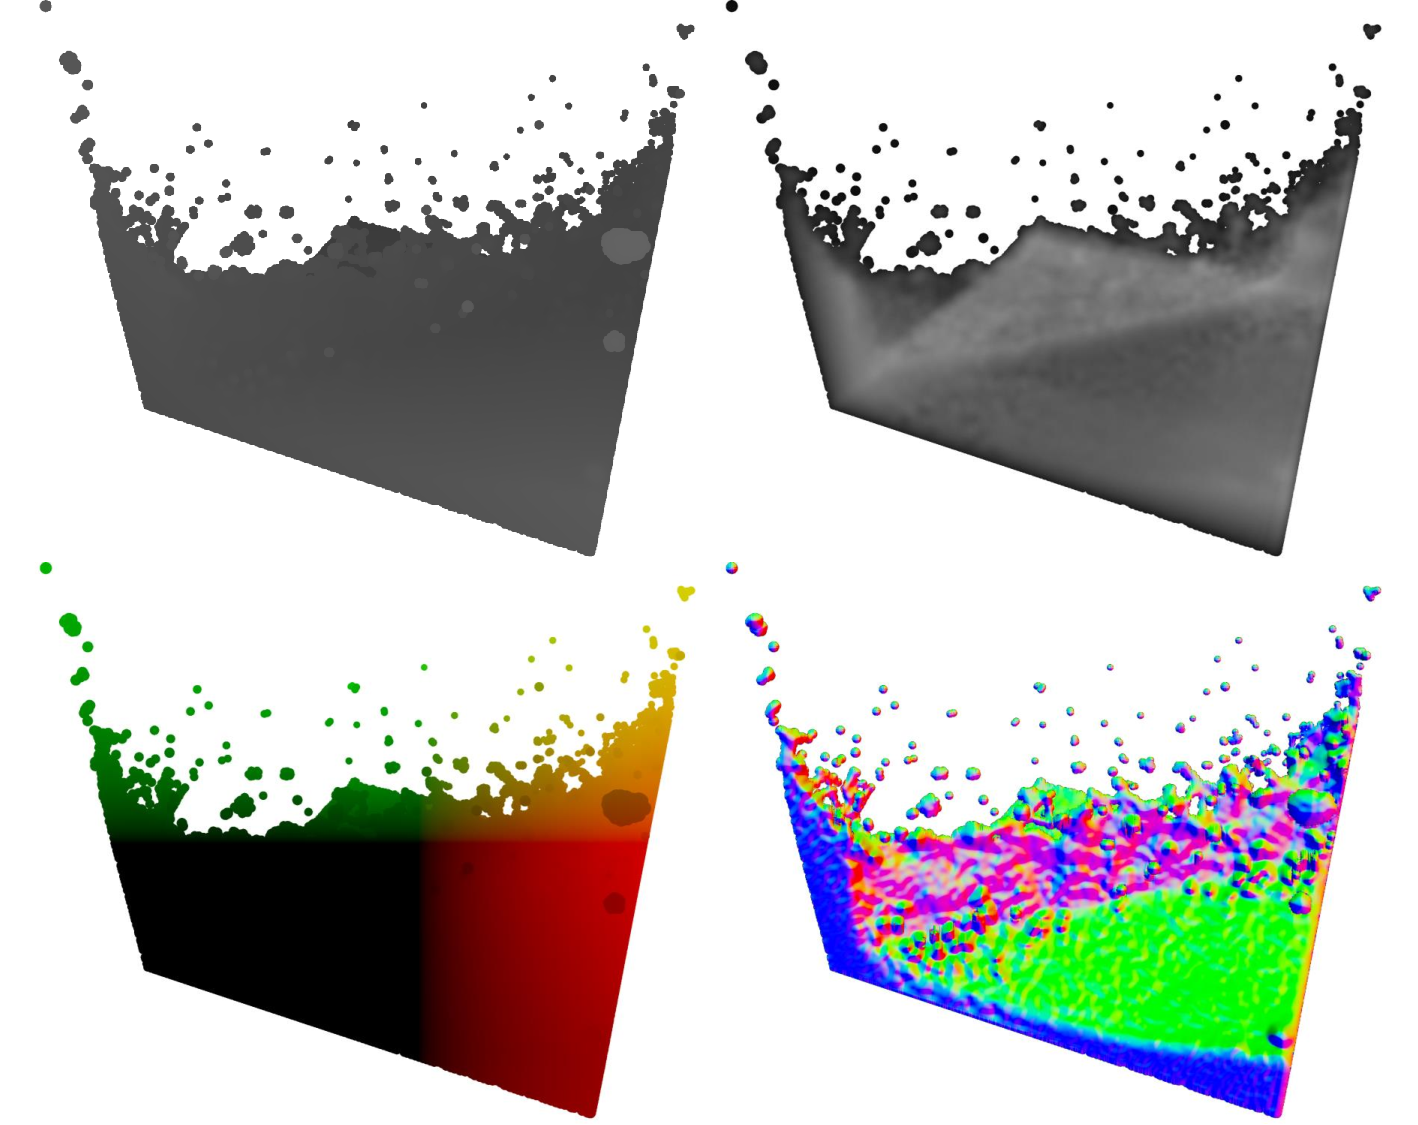
\includegraphics[width=.8\textwidth]{figures/rendering/d_t_p_n.pdf}
    	\caption{深度图(左上)厚度图(右上)位置还原效果(左下)法向还原效果(右下)}
        \label{fig:dtpn}
    \end{figure}
    
    综合公式6-3与公式6-4,采样点深度值在窄域范围内时滤波核权重与高斯核相同,但是在深度过浅时会将其贡献忽略调。但是直接忽略采样值会导致滤波核不对称,在流体表面法向与视线方向相差角度越大时,计算偏差越明显。为了解决这一问题,可以将深度过浅的采样点 $j$ 的对称位置 $k$ 的深度贡献同时忽略($\mathbf{u}_k = 2\mathbf{u}_i - \mathbf{u}_j$),以保证滤波核的对称性,调整之后滤波核的定义为
    \begin{equation}
    	\omega_{ij} =
    	\left\{
    	\begin{array}{ll}
    	0, 											& \mathrm{if} \ z_j > z_i + \delta \ \mathrm{or} \ z_k > z_i + \delta \\
    	G(\mathbf{u}_i, \mathbf{u}_j, \sigma_i),   	& \mathrm{otherwise} \\
    	\end{array}
    	\right.
    \end{equation}
    
    根据公式6-2与公式6-3,可以得到窄域范围的定义为 $z_i + \delta \ge z_j \ge z_i - \delta$。全局所有滤波点均使用这一窄域范围,显然这样定义是不准确的,因为流体表面深度的变化率差异较大,所以需要针对每个滤波点调整窄域范围。具体来说,可以在滤波过程中迭代调整窄域范围,设迭代过程中窄域定义为 $z_i + \delta_{high} \ge z_j \ge z_i - \delta_{low}$,其迭代初始值均设为 $\delta$,迭代策略为
    \begin{equation}
    	\begin{gathered}
    	\delta_{high} \leftarrow \max (\delta_{low}, z_i - z_j + \delta) \\
    	\delta_{low} \leftarrow \max (\delta_{low}, z_j - z_i + \delta)
    	\end{gathered}
    \end{equation}
    
    在具体实现上,由于2D滤波的效率在实时渲染中的计算量是不可接受的,所以本文将其拆分为x方向和y方向的两个1D滤波,不过在数学上这并不等价,会在流体轮廓边缘处造成轻微瑕疵。1D滤波核宽度设置为32像素,$\sigma$ 为1/4滤波核宽度,$\delta$ 为5倍粒子半径,$\mu$ 等于粒子半径。
    
    \begin{figure}
    	\centering
    	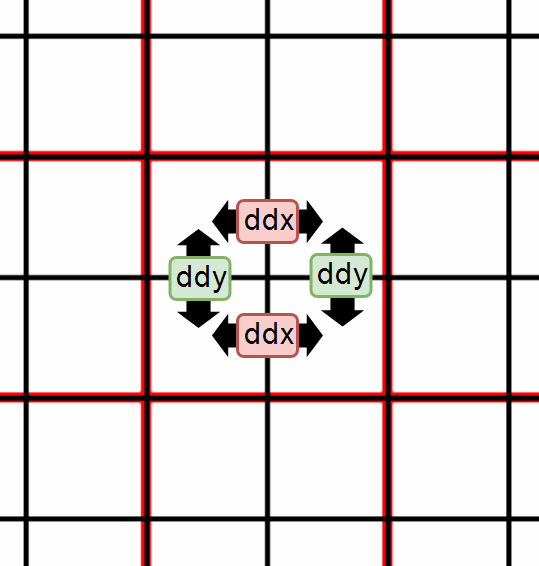
\includegraphics[width=.25\textwidth]{figures/rendering/ddx_ddy.png}
    	\caption{一阶差分}
    	\label{fig:difference}
    \end{figure}

\subsection{屏幕空间渲染}
    至此,得到平滑深度图与厚度图之后,就需要根据每个像素的深度、厚度、位置以及环境光信息完成着色。
    
    首先需要从深度 $z$ 与像素在平面上的位置 $[u,v]$ 还原其对应流体表面在相机坐标系下的位置坐标以及表面法向量。位置坐标可以很容易的通过像素位置与相机参数(屏幕分辨率 $[W, H]$,相机近平面距离 $n$)得到
    \begin{equation}
    	\mathbf{p} = z \
    	\left[
    	\frac{(u - 0.5) W} {n}, \;
    	\frac{(0.5 - v) H}{n}, \;
    	-1
    	\right]^T
    \end{equation}
    
    \begin{figure}
    	\centering
    	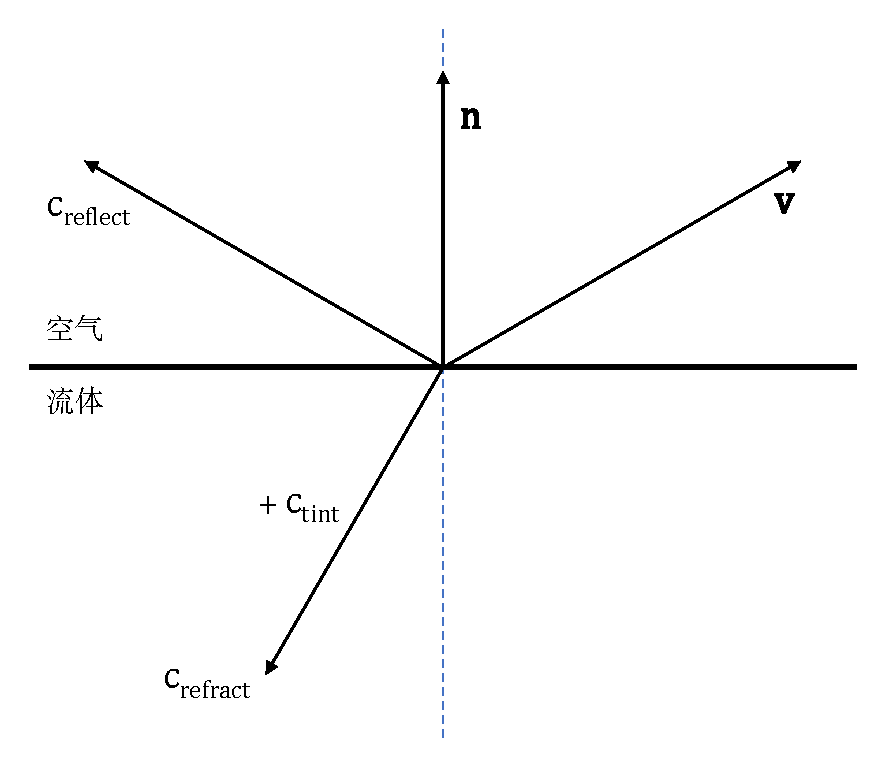
\includegraphics[width=.35\textwidth]{figures/rendering/shading.pdf}
    	\caption{反射与折射方向}
    	\label{fig:refraction}
    \end{figure}
    
    而法向可以看作流体表面两个不同的切线方向的叉乘,比如x方向和y方向。而切线又可以由流体表面位置的偏微分得到,所以法向的计算公式为
    \begin{equation}
    	\mathbf{n} = \frac {\partial \, \mathbf{p}} {\partial \, x} \times \frac {\partial \, \mathbf{p}} {\partial \, y}
    \end{equation}
    
    在硬件光栅化时,GPU往往会以 $2\times 2$ 的像素块为一个线程组进行计算,这样可以非常方便得在线程组内通过一阶差分近似偏微分(如图\ref{fig:difference})。同样,WebGPU在像素着色器中提供了偏微分内置函数dpdx()与dpdy(),所以我们可以非常容易地还原法向值,代码如下。

    \begin{listing}[htbp]
    \begin{minted}{glsl}
    fn getNormal(positionEye: vec3<f32>) -> vec3<f32> {
        let ddx = dpdx(positionEye);
        let ddy = dpdy(positionEye);
        let normalEye = normalize(cross(-ddx, ddy));
        return normalEye;
    }
    \end{minted}
    \caption{从深度图还原法向的wgsl着色器代码}
    \label{code:normal}
    \end{listing}
    
    在得到完整的几何信息之后,就可以进一步完成着色了。首先通过表面法向 $\mathbf{n}$ 和视线方向 $\mathbf{v}$ 计算菲涅尔项 $F$,它确定了在物体表面光线折射与反射的能量比值,本文采用了经典的Schick近似的菲涅尔计算公式\cite{S94BRDF}
    \begin{equation}
    	\begin{gathered}
    	F = F_0 + (1 - F_0) (1 - (\mathbf{n} \cdot \mathbf{v})^+)^5 
    	\\
    	F_0 = (\frac{n - 1}{n + 1})^2
    	\end{gathered}
    \end{equation}
    其中 $n$ 为物体表面折射率,代入水的折射率1.33可得 $F_0 \approx 0.02$ 。
    
    然后,我们可以根据反射和折射定律得到光线反射与折射方向,以这两个方向分别采样环境光贴图,即可得到流体表面的反射颜色 $c_{reflect}$ 与折射颜色 $c_{refract}$ 。折射颜色还需进一步与流体本征颜色 $c_{tint}$ 根据流体厚度衰减系数 $\gamma$ 进行插值(如图\ref{fig:refraction})。最后,以菲涅尔项 $F$ 确定反射颜色与折射颜色的比值,将其混合输出
    \begin{equation}
    	\begin{gathered}
    	c = \mathrm{lerp} ( \mathrm{lerp} (c_{tint},\ c_{refract},\ \gamma),\ c_{reflect},\ F ) 
    	\\
    	\gamma = exp(-t)
    	\end{gathered}
    \end{equation}
    
    \begin{figure}[htbp]
    	\centering
    	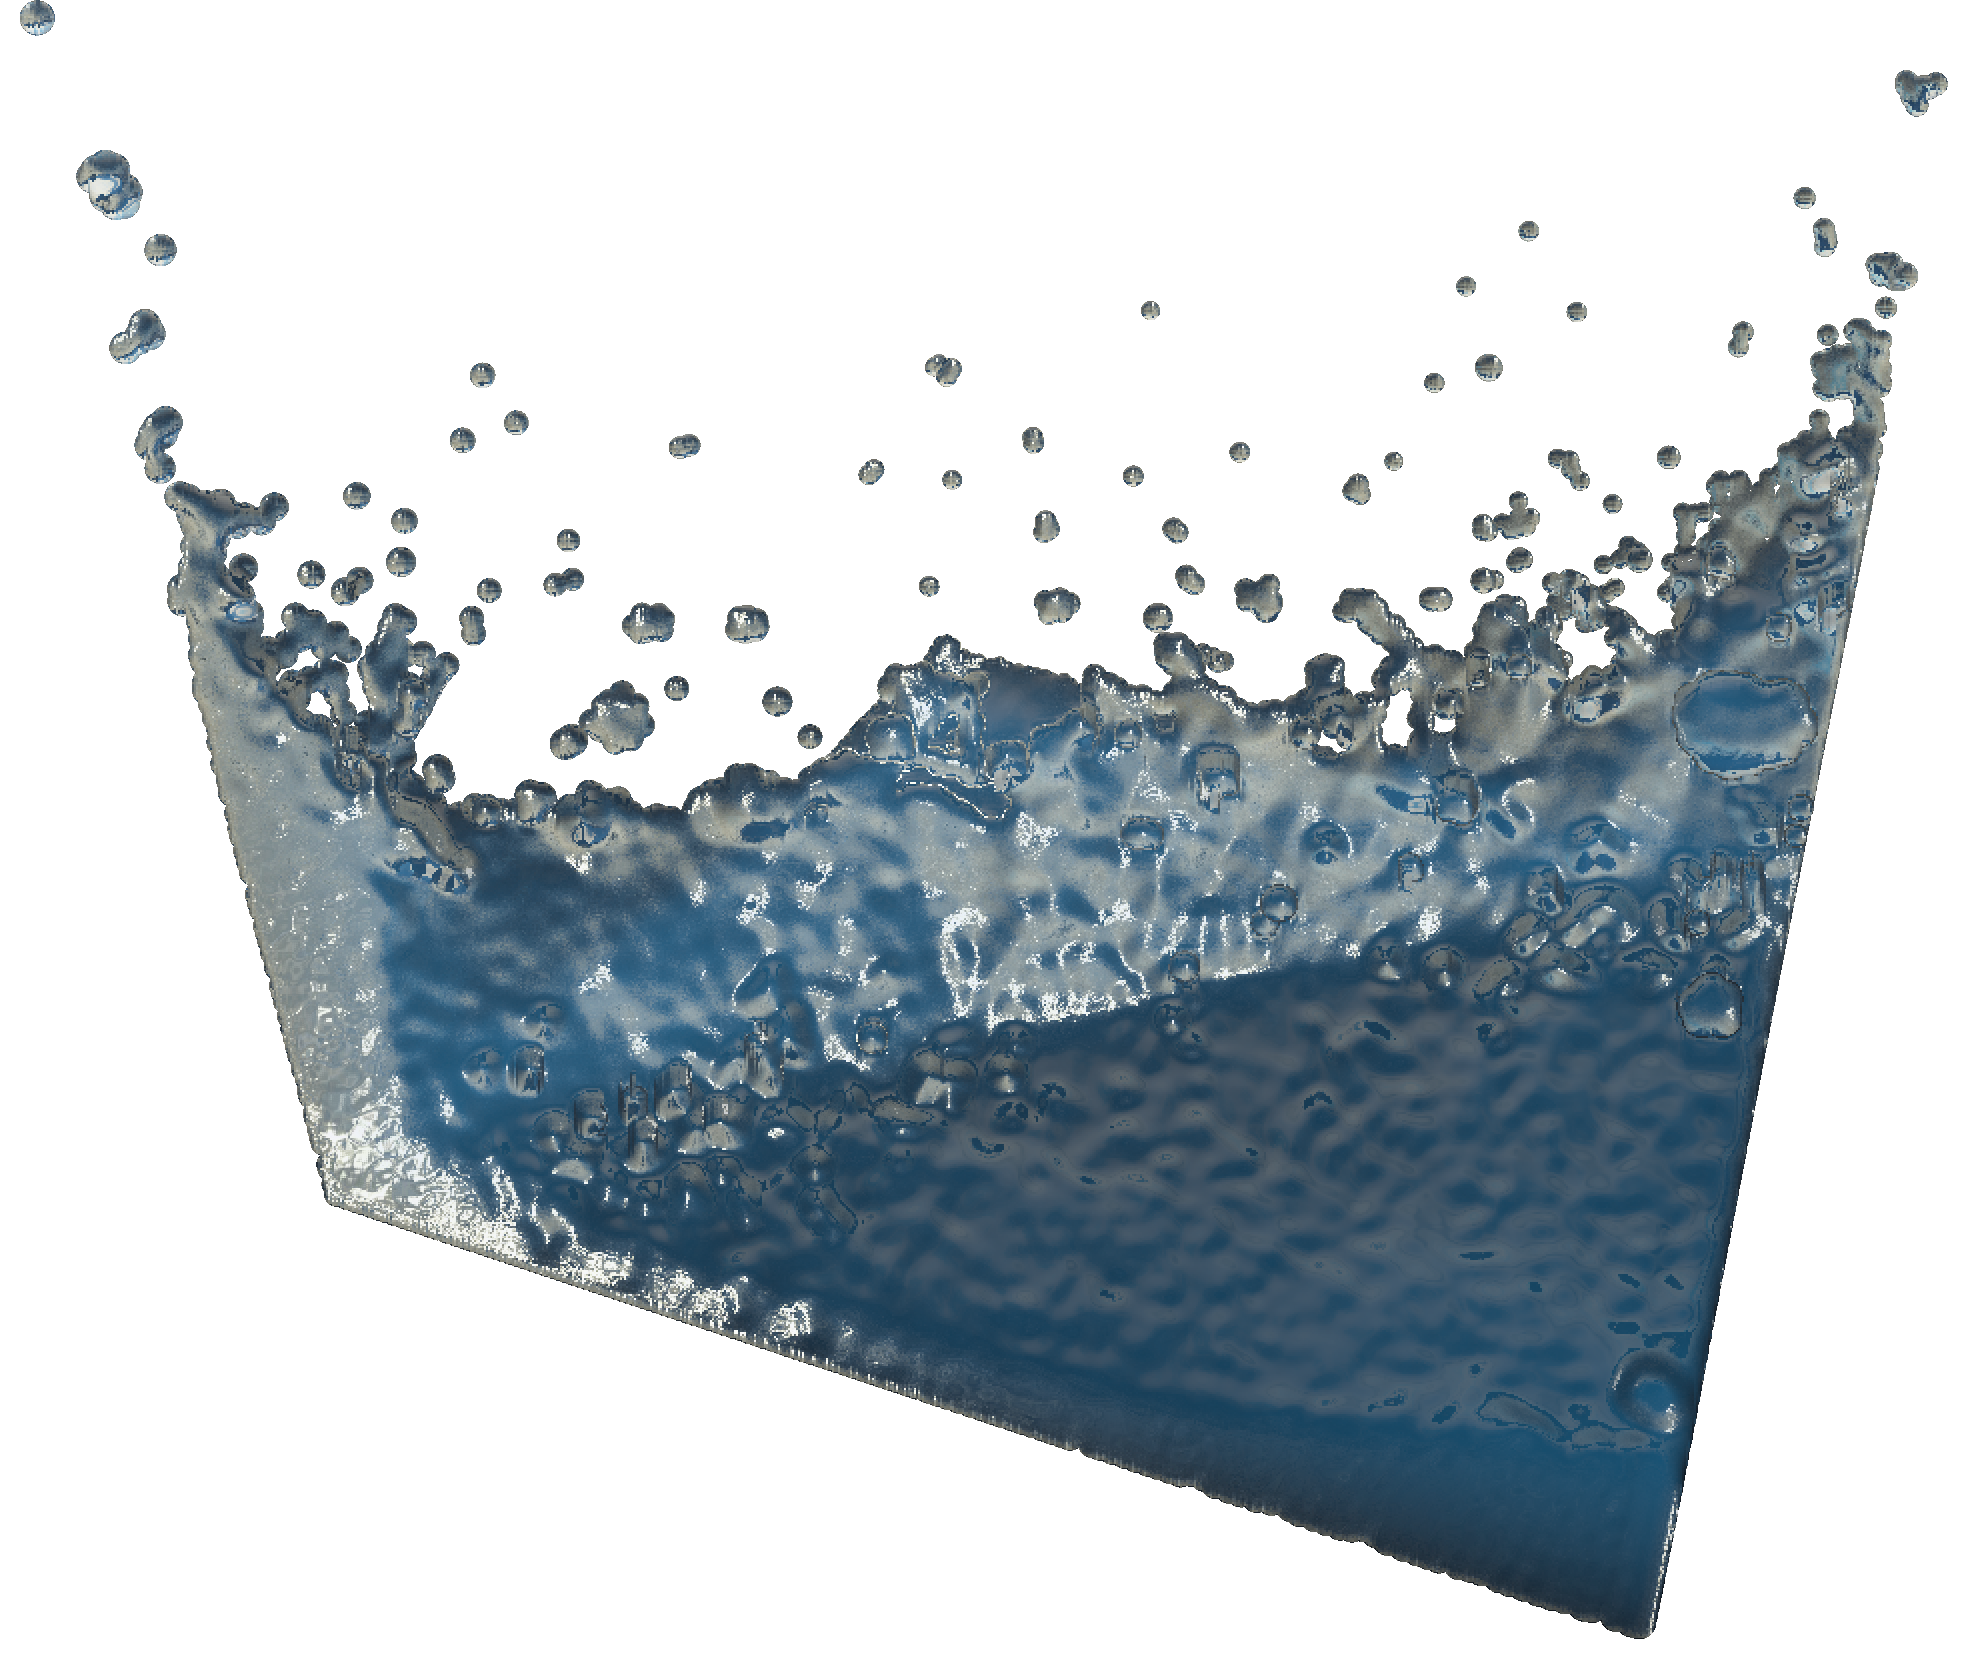
\includegraphics[width=.6\textwidth]{figures/rendering/result.png}
    	\caption{渲染结果}
    \end{figure}

\subsection{本章小结}
本章主要阐述了流体仿真系统的渲染部分的原理与实现。我们将物理模拟的结果——流体粒子,通过实例化渲染得到深度图与厚度图,再使用窄域滤波器平滑深度图,最后在屏幕空间完成流体渲染。相应地,在实现中我们使用WebGPU渲染-计算-渲染的混合管线架构,在实时物理模拟计算的同时完成高质量渲染,帧数几乎没有下降,这全面体现了WebGPU带来的新特性与性能优势。